\section{Triangle Geometry}

\subsection{Signed Lengths and Orientation}

A line through two points \(A\) and \(B\) is denoted \(AB\), typically \textit{in that direction}. For a point \(P\) on the line \(AB\), if \(P\) lies between \(A\) and \(B\) then the ratio \(\frac{AP}{PB} > 0\). But if \(P\) is outside \(A\) and \(B\) then \(\frac{AP}{PB} < 0\). If \(P\) and \(A\) are the same point, then the ratio is zero; if \(P\) and \(B\) are the same, then the ratio is \(\infty\). \\

An \textbf{altitude} of a triangle is a line segment through a given vertex and perpendicular to the line containing the side opposite the vertex. \\

In a triangle, the orientation is called \textbf{positive} if the vertices are taken anti-clockwise in the order given. For an oriented triangle, we take directed lengths to match the orientation: \(AB, BC\) and \(CA\) are positive in \(\triangle ABC\). We extend this convention to area and angle:
\begin{itemize}
    \item The area of a triangle is positive if the triangle is positively oriented; otherwise it is negative.
    \item Positive angles go anticlockwise. If edges are signed, we need to account for that. We take \(\angle ABC\) as positive if the sense runs anticlockwise from \(BA\) to \(BC\) when both are the same sign; if they are opposite signs, we change the sign of the angle to compensate.
\end{itemize}

We denote the sign of the area as \(\triangle ABC = \frac{1}{2} |AB| \cdot |BC| \cdot \sin ABC\).

\subsection{Intersections}

A \textbf{centroid} is the intersection of the medians while a \textbf{orthocetnre} is the intersection of altitudes. It can be shown that the medians are concurrent. The medians and altitudes are examples of \textbf{cevians}.

\defn{Cevian}{
    In any triangle a line segment joining a vertex to a non-vertex point on the opposite side, possibly extended, is called a cevian.
}

\thrm{Ceva's Theorem (1678)}{
    In \(\triangle ABC\) the cevians \(AD, BE\) and \(CF\) (where \(D\) is on \(BC\), \(E\) is on \(AC\) and \(F\) is on \(AB\)) are concurrent if and only if
    \[\frac{AF}{FB} \cdot \frac{BD}{DC} \cdot \frac{CE}{EA} = 1.\]
}

\begin{corollary}
    In \(\triangle ABC\) the cevians \(AD, BE\) and \(CF\) are concurrent if and only if
    \[\frac{\sin ACF}{\sin FCB} \cdot \frac{\sin BAD}{\sin DAC} \cdot \frac{\sin CBE}{\sin EBA} = 1,\]
    taking proper account of orientations of the angles.
\end{corollary}

\subsection{Collinearity}

\thrm{Menelaus' Theorem}{
    In \(\triangle ABC\) let \(D, E\) and \(F\) be on side \(BC, CA, AB\) (or their extensions) respectively. Then \(D, E\) and \(F\) are collienar if and only if
    \[\frac{AF}{FB} \cdot \frac{BD}{DC} \cdot \frac{CE}{EA} = -1.\]
}

\thrm{Pappus' Theorem}{
    Suppose points \(A, C, E\) lie on one line and \(B, D, F\) on a second line, where \(AB, CD\) and \(EF\) form a triangle. Let \(L = AB \cap DE, M = CD \cap FA\) and \(N = EF \cap BC\). Then \(L, M\) and \(N\) are collinear.
}

\subsection{Angle Bisectors}

\defn{Bisectors}{
    In the image below, the line \(AP\) in the left hand diagram is the \textbf{internal bisector} of \(\angle BAC: \angle BAP = \frac{1}{2} \angle BAC\) and the line \(AQ\) in the right hand diagram is the \textbf{external bisector} of \(\angle BAC: \angle CAQ = \frac{1}{2}(\pi - \angle BAC)\), that is it bisects angle between \(AC\)and the extension of the line \(AB\).
    \begin{center}
        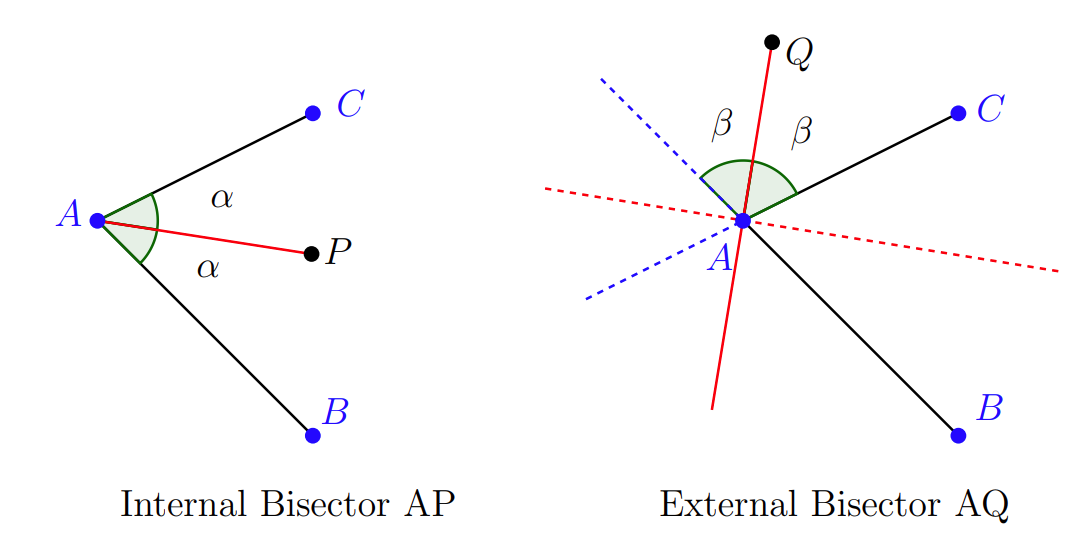
\includegraphics{assets/triangle/bisectors.png}
    \end{center}
}

\thrm{Angle Bisector Theorem}{
    Consider \(\triangle ABC\), and its angle bisector as below.
    \begin{enumerate}[label=\alph*)]
        \item If the interior bisector of \(\angle BAC\) meets \(BC\) at \(P\) then \(\frac{BP}{PC} = \frac{AB}{CA}\).
        \item If the exterior bisector of \(\angle BAC\) meets \(BC\)at \(Q\)then \(\frac{BQ}{QC} = -\frac{AB}{CA}\).
    \end{enumerate}
    \begin{center}
        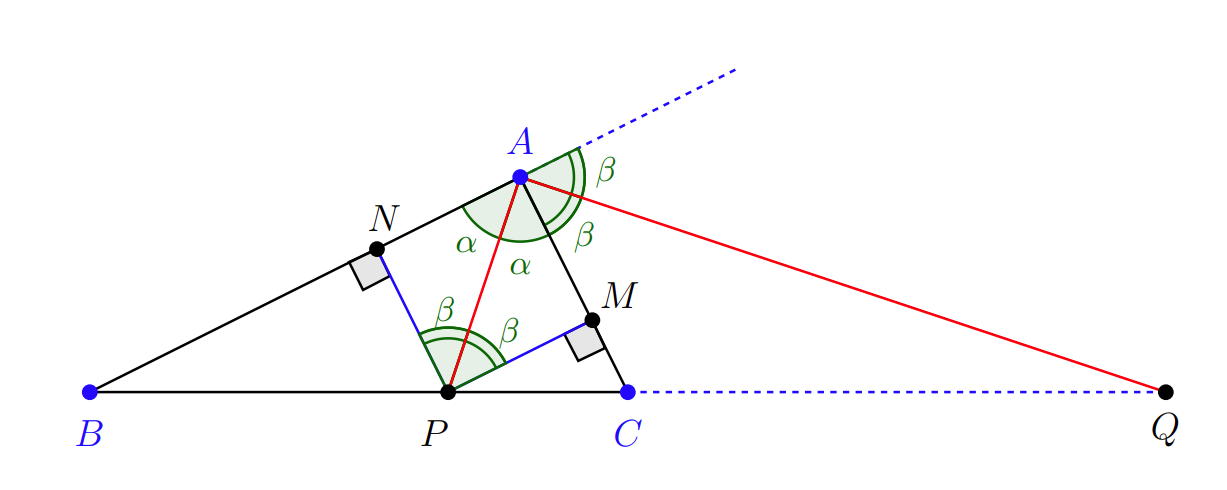
\includegraphics{assets/triangle/bisector_theorem.png}
    \end{center}
}

\thrm{Incentre Theorem}{
    The internal bisectors of a triangle are concurrent.
}

The point of concurrence is called the \textbf{increntre}. This point is equidistance from the three sides, so a circle centred here and tangent to the edges is the largest circle that can fit inside the triangle. This circle is called the \textbf{incircle}.

\thrm{Excentre Theorem}{
    The external bisectors of any two angles of a triangle are concurrent with the internal bisector of the third angle.
}

The points of concurrence (there are three of them) are called the \textbf{excentres}. Again, each excentre is the same distance from the three sides, and so circles centres at the excentres with that distance as radius (the \textbf{excircles}) are tangent to the sides of the triangle, one internally, two externally.


\begin{theorem}
    In \(\triangle ABC\), let the internal bisectors at angles \(A, B\) and \(C\) meet the opposite sides at \(P, Q\) and \(R\) respectively and the external bisectors meet the opposite sides at \(P', Q'\) and \(R'\) respectively. Then \(\{P, Q, R'\}, \{P, Q', R\}\) and \(\{P', Q, R\}\) are triples of collinear points.
\end{theorem}

\subsection{Area Formulas}

Let \(r\) be the radius of the incircle. Then
\[\triangle ABC = \frac{1}{2}r(a + b + c) = sr,\]
where \(s = \frac{1}{2}(a + b + c)\) is the semiperimeter. \\

We can get similar results from the excircles. Let \(r_a\) be the radius of the excircle centred at \(J_a\). Then
\[\triangle BCJ_a = \frac{1}{2}r_a \cdot a, \quad \triangle ABJ_a = \frac{1}{2}r_a \cdot c, \quad \triangle ACJ_a = \frac{1}{2}r_a \cdot b,\]
since \(r_a\) is the distance to each edge. Thus,

\[\triangle ABC = \frac{1}{2}r_a(b - a + c) = (s - a)r_a.\]

Then similarly, we have

\[\triangle ABC = (s - b)r_b = (s - c)r_c.\]

After some trigonometry and rearranging to solve for \(r\), we get

\[r = \sqrt{\frac{(s - a)(s - b)(s - c)}{s}}.\]

Then from the previous expression we get \textbf{Heron's formula}:

\[\triangle ABC = \sqrt{s(s - a)(s - b)(s - c)}.\]

Then we get the following results,

\[r_a = \sqrt{\frac{s(s - b)(s - c)}{s - a}} \qquad \text{ and } \qquad \frac{1}{r} = \frac{1}{r_a} + \frac{1}{r_b} + \frac{1}{r_c}.\]

\subsection{Circles Associated to Triangles}

The \textbf{circumcircle} goes through the three vertices of a triangle and has centre the \textbf{circumcentre}, the intersection of the three perpendicular bisectors of the sides. \\

Suppose for a circle \(\triangle ABC\) with circumcentre \(O\). Let \(OA = OB = OC = R\) be the \textbf{circumradius}. Then \(\angle AOB = 2\angle C\) and so \(\angle C = \angle FOB\). Thus \(R\sin C = FB = \frac{c}{2}\). Then similar results for the other sides gives the \textbf{extended sine rule}:
\[\frac{a}{\sin A} = \frac{b}{\sin B} = \frac{c}{\sin C} = 2R.\]

\begin{lemma}
    The circumcentre of a triangle is the orthocentre of its median triangle.
\end{lemma}

\thrm{Nine Point Circle}{
    For \(\triangle ABC\), let \(A', B'\) and \(C'\) be the midpoints of the three sides and \(H_a, H_b\) and \(H_c\) be the feet of the altitudes. Let \(H\) be the orthocentre and \(E_a, E_b\) and \(E_c\) be the midpoints of the lines from \(H\) to the three vertices. Also let \(O\) be the circumcentre and \(R\) the circumradius. Then if \(N\) is the midpoint of the line from \(H\) to \(O\), the nine points \(A', B', C', H_a, H_b, H_c, E_a, E_b\) and \(E_c\) lie on the circle centre \(N\) of radius \(\frac{R}{2}\).

    \begin{center}
        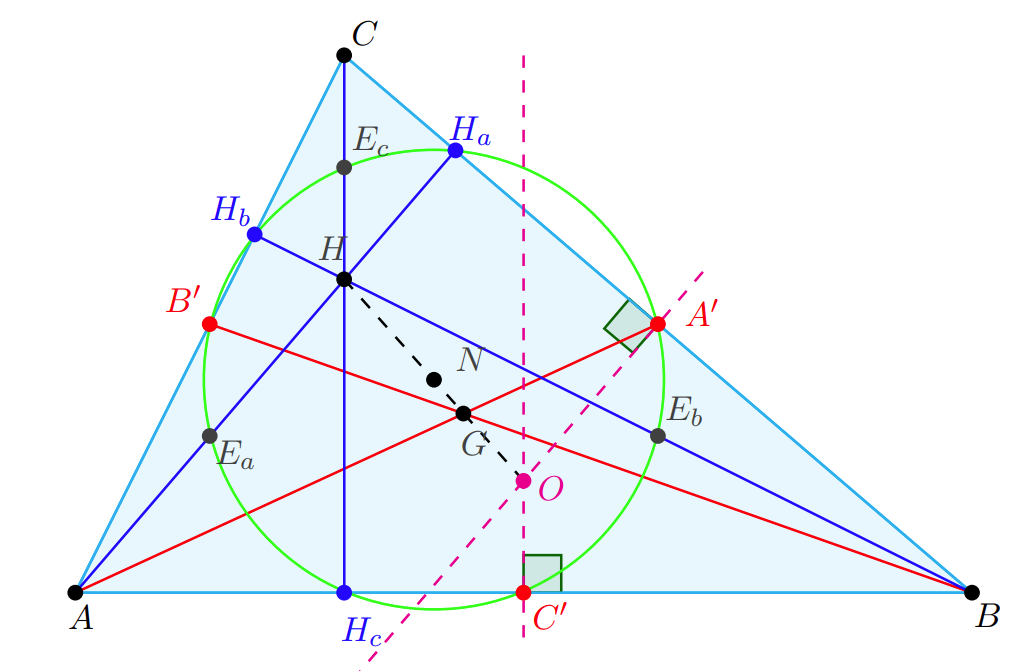
\includegraphics{assets/triangle/nine_point_circle.png}
    \end{center}
}

\thrm{Feuerbach's Theorem}{
    The nine-point circle is tangent to the incircle and all three excircles.
}

The point where the incircle and the nine-point circle meet is called the \textbf{Feuerbach point}. It is collinear with the incentre and the nine-point centre.

\thrm{The Euler Line}{
    In any triangle, the orthocentre \(H\), nine-point centre \(N\), circumcentre \(O\) and centroid \(G\) are collinear. Furthermore \(N\) is the midpoint \(OH\) and \(OG : GH = 1 : 2\).
}

The line these points lie on is called the \textbf{Euler Line}.

\thrm{Simson Line}{
    Let \(P\) be any point on the circumcirle of \(\triangle ABC\). Then the feet of the perpendiculars from \(P\) to each side of \(\triangle ABC\) are collinear.
}

\begin{proposition}
    The three Euler points uniquely define a triangle.
\end{proposition}

\subsection{The Cross Ratio}

\begin{theorem}
    Let \(\triangle ABC\) have points \(D, E, F\) on the sides opposite \(A, B, C\) respectively and suppose the cevians \(AD, BE\) and \(CF\) are concurrent at a point \(P\) inside \(\triangle ABC\). Let \(Q\) be a point on \(BC\).

    Then \(F, E\) and \(Q\) are collinear if and only if \(\displaystyle{\frac{BD \cdot CQ}{CD \cdot BQ} = -1}\).
\end{theorem}

\defn{Cross Ratio}{
    Let \(A, B, C, D\) be any four points. The cross ratio \((A, B; C, D)\) is defined by
    \[(A, B; C, D) = \frac{AC}{BC} \divisionsymbol \frac{AD}{BD} = \frac{AC \cdot BD}{BC \cdot AD}.\]
}

Note that changing the order of the points in \((A, B; C, D)\) may change the value of the cross ratio. However

\[(A, B; C, D) = (B, A; D, C) = (C, D; A, B) = (D, C; B, A),\]

so there are at most 6 different values of the cross ratio.

\defn{Harmonic}{
    A set of collinear points \(\{A, B, C, D\}\) for which \((A, B; C, D) = -1\) are said to be harmonic, and \(C, D\) are called the harmonic conjugates of \(A, B\).
}

\begin{theorem}
    In the diagram below, we have \\
    \begin{minipage}{0.3\textwidth}
        \begin{center}
            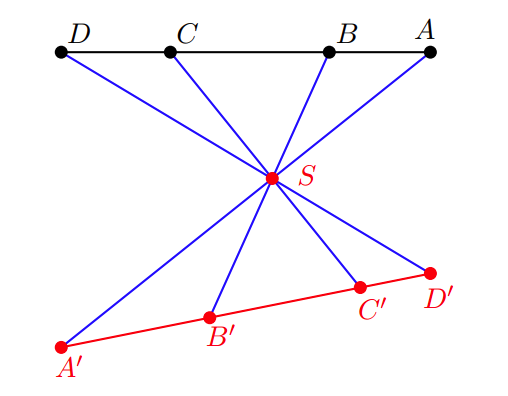
\includegraphics{assets/triangle/cross_product_angles.png}
        \end{center}
    \end{minipage}
    \hfill
    \begin{minipage}{0.65\textwidth}
        \[(A, B; C, D) = (A', B'; C', D') = \left(\frac{\sin \angle ASC}{\sin \angle BSC}\right) \cdot \left(\frac{\sin \angle BSD}{\sin \angle ASD}\right).\]
    \end{minipage}
\end{theorem}

The sets \(\{A, B, C, D\}\) and \(\{A', B', C', D'\}\) are said to be in perspective from \(S\), or one set if projected from \(S\). Our result can then be stated as the cross ratio of collinear points is a projective invariant.

\begin{theorem}
    \setlength{\parindent}{1em}
    Suppose that in \(\triangle ABC, X\) and \(Y\) are points on \(AB\) such that \(CX\) is the internal bisector of \(\angle ACB\) and \(CY\) its external bisector. Then \((A, B; X, Y) = -1\), i.e. the four points are harmonic.

    Conversely, given points \(X\) and \(Y\) on side \(AB\) of \(\triangle ABC\) with \(CX\) orthogonal to \(CY\), if \((A, B; X, Y) = -1\) then \(CX\) is the internal and \(CY\) the external bisector of \(\angle ACB\).
\end{theorem}
